\section{Energização de linhas e rejeição de carga}

A energização da linha pode ser representada pelo emprego de quadripolos ou do modelo de circuito $\pi$. A energização se dá considerando a inexistência de carga no final da linha e pode ser representado pelo quadripolo da figura \ref{top2:fig:1}.

\begin{figure}[H]
\begin{center}
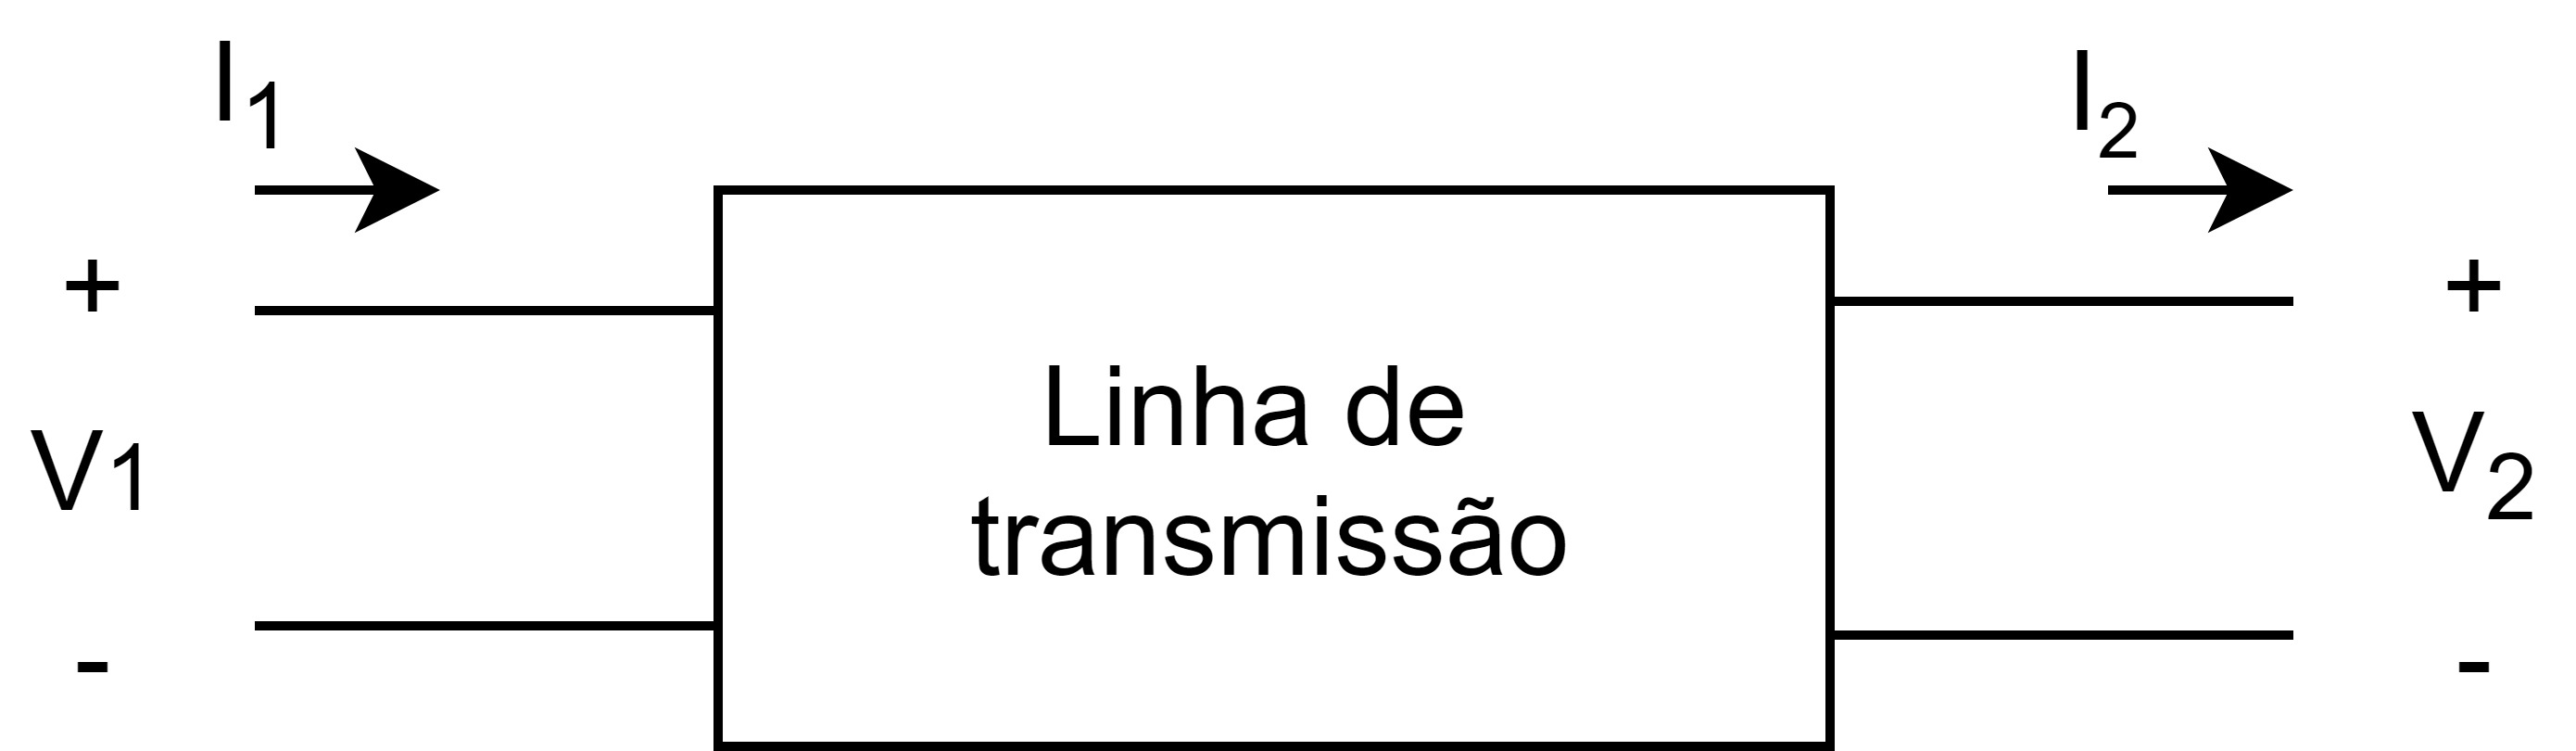
\includegraphics[width=8cm]{images/quadripolo.jpg}
\caption{Quadripolo base para as análises. Fonte: própria.}
\label{top2:fig:1} 
\end{center}
\end{figure}

Considerando a corrente e tensão de entrada do quadripolo como $I_1$ e $V_1$, respectivamente e a corrente e tensão de saída como $I_2$ e $V_2$, respectivamente, a equação \ref{top2:eq:1} representa a relação entre entrada e saída, mediada pela matriz de coeficientes do quadripolo tomadas no ponto $s = j\omega$. As constantes do quadripolo vão depender do tipo de modelo utilizado para representar a linha. 

\begin{equation} \label{top2:eq:1}
    \begin{bmatrix} V_1 \\ I_1  \end{bmatrix} \,=\, \begin{bmatrix} A & B \\ C_q & D  \end{bmatrix}\, \begin{bmatrix} V_2 \\ I_2  \end{bmatrix}
\end{equation}

Para uma análise generalizada, observa-se que para uma linha em vazio ($I_2=0$), a sobretensão pode ser avaliada pela relação: $V_1 = AV_2$. De forma que, determinando a constante generalizada A da linha de acordo com o modelo em questão, a sobretensão de energização poderá ser quantificada.

Os modelos de representação de linha são os modelos: de linha curta, linha média e linha longa; e estes devem ser utilizados de forma adequada à aplicação para permitir um esforço computacional menor e resultados com alta confiabilidade.

\begin{itemize}
    \item Linha curta
\end{itemize}

O modelo de linha curta é utilizado para linhas de transmissão de comprimento até 80 km e o modelo não possui frequência de ressonância. 

O circuito equivalente para esse tipo de linha é representado na figura \ref{top2:fig:2} e ele mostra que apenas é representada a impedância longitudinal da linha, assim desprezando a admitância transversal da linha. Em resumo, pode-se dizer que nesse modelo o efeito capacitivo com a terra é desprezando, logo considerando apenas o efeito resistivo e indutivo da linha. 

\begin{figure}[H]
\begin{center}
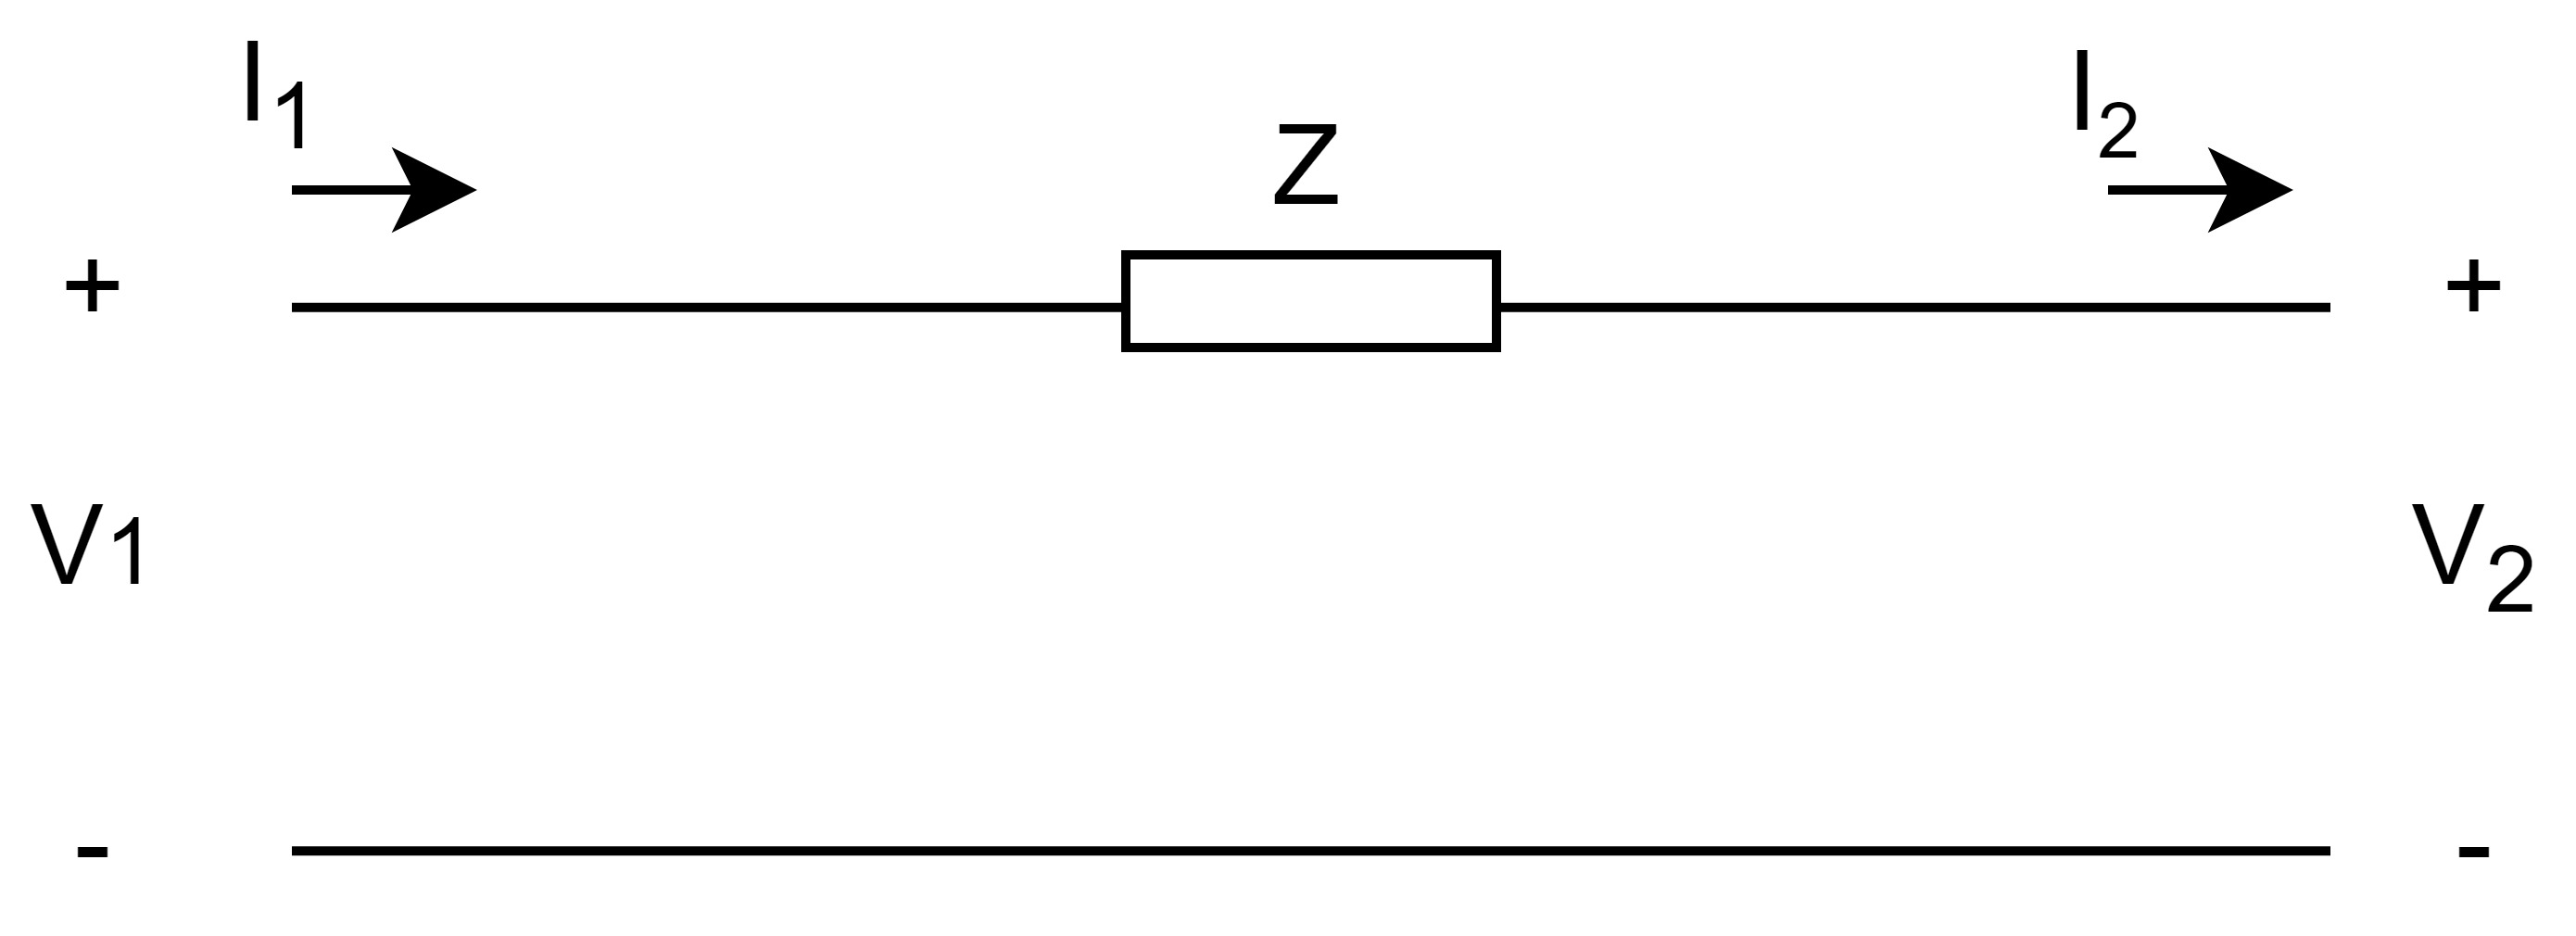
\includegraphics[width=8cm]{images/linha_curta.jpg}
\caption{Modelo de linha curta. Fonte: própria.}
\label{top2:fig:2} 
\end{center}
\end{figure}

Por meio do quadripolo da figura \ref{top2:fig:2} é possível estabelecer as relações entre tensões e correntes e aplicá-las na forma matricial, assim tem-se que:

\begin{equation} \label{top2:eq:3}
    \begin{bmatrix} V_1 \\ I_1  \end{bmatrix} \,=\, \begin{bmatrix} 1 & Z \\0 & 1  \end{bmatrix}\, \begin{bmatrix} V_2 \\ I_2  \end{bmatrix}
\end{equation}

\begin{itemize}
    \item Linha média
\end{itemize}

Já o modelo de linha média é aplicado para linhas maiores que a linha curta, mas até 240 km de comprimento e o modelo possui uma frequência de ressonância. 

A figura \ref{top2:fig:3} permite observar que esse modelo de linha difere do anterior devido a adição de uma admitância \textit{shunt} para modelar o efeito capacitivo que se torna muito mais evidente em linhas de transmissão desta magnitude.

\begin{figure}[H]
\begin{center}
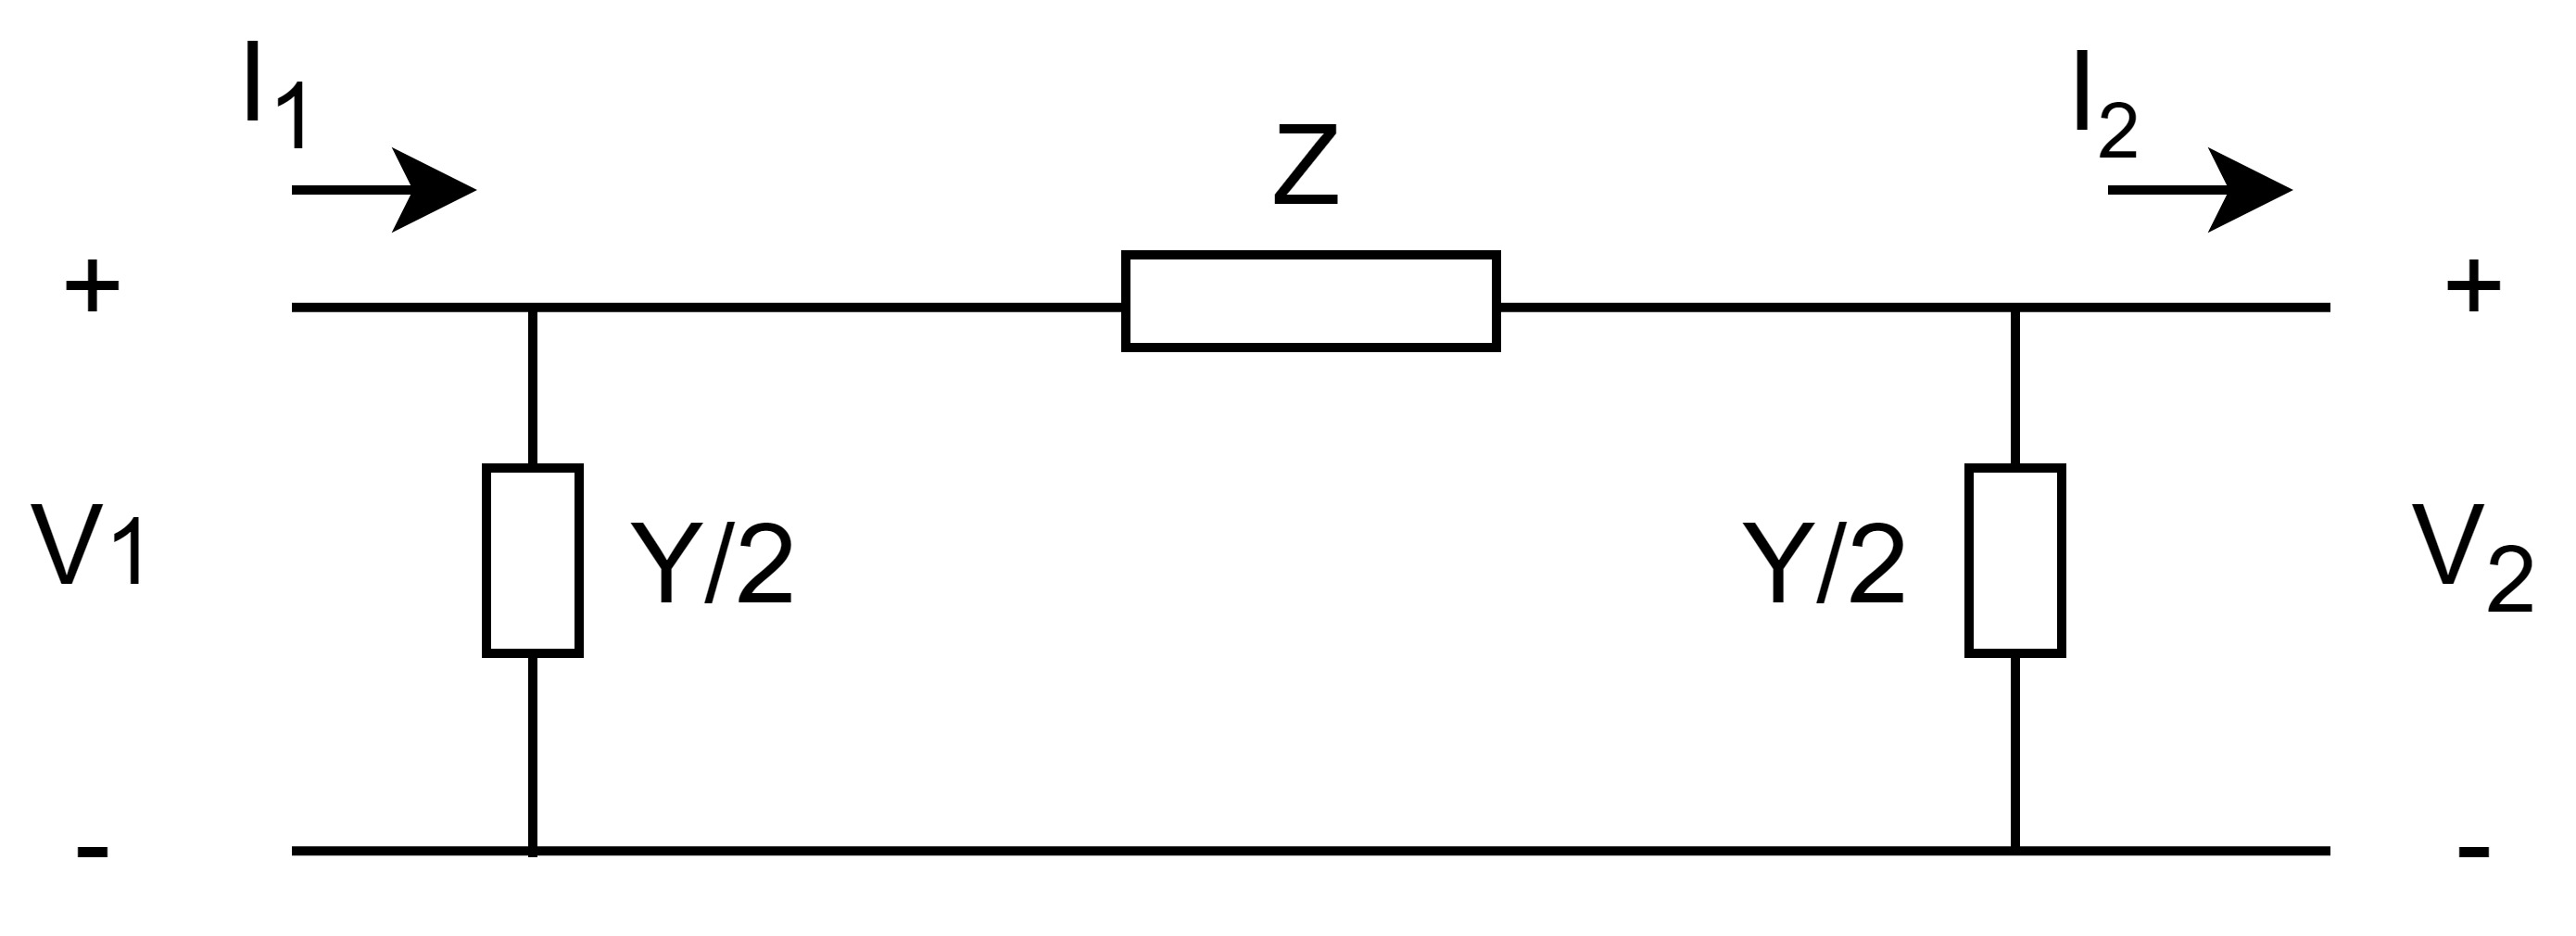
\includegraphics[width=8cm]{images/linha_media.jpg}
\caption{Modelo de linha média. Fonte: própria.}
\label{top2:fig:3} 
\end{center}
\end{figure}

Por meio do quadripolo da figura \ref{top2:fig:3} é possível estabelecer as relações entre tensões e correntes na forma matricial da equação \ref{top2:eq:4}. 

\begin{equation} \label{top2:eq:4}
    \begin{bmatrix} V_1 \\ I_1  \end{bmatrix} \,=\, \begin{bmatrix} \frac{ZY}{2}+1 & Z \\ Y\left(\frac{ZY}{4}+1\right)  & \frac{ZY}{2}+1  \end{bmatrix}\, \begin{bmatrix} V_2 \\ I_2  \end{bmatrix}
\end{equation}


\begin{itemize}
    \item Linha longa
\end{itemize}

As linhas longas são consideradas qualquer uma que possua comprimento maior que 240 km. Para a sua análise é utilizado o modelo de parâmetros distribuídos. Assim, cada trecho infinitesimal da linha será representado pelo modelo de linha média com elementos infinitesimais de corrente e tensão a cada trecho. A solução da equação diferencial resultante resulta na equação \ref{top2:eq:5} na forma matricial (a demonstração dessa fórmula foi foco da disciplina de análise de sistemas de potência 2).  

\begin{equation} \label{top2:eq:5}
    \begin{bmatrix} V_1 \\ I_1  \end{bmatrix} \,=\, \begin{bmatrix} cosh(\gamma l) & Z_c senh(\gamma l) \\ \frac{1}{Z_c}senh(\gamma l) & cosh(\gamma l)  \end{bmatrix}\, \begin{bmatrix} V_2 \\ I_2  \end{bmatrix}
\end{equation}

É intuitivo que o uso do modelo de linha longa para casos de linha curta ou média resultarão em resultados satisfatórios. Porém, esse modelo requer muita carga computacional, de forma que o erro gerado em comparação com o uso do modelo correto é pequeno o suficiente para restringir esse modelo apenas para casos realmente necessários.

Observa-se que para uma linha curta a constante generalizada A sempre terá valor unitário ($A=1$), implicando em uma sobretensão desprezível. Porém, no caso da linha média e longa essa constante será menor que a unidade ($A<1$), necessitando de compensação para que a sobretensão resultante não seja prejudicial para o sistema.

\subsection{Consumo e compensação de reativo}

Devido a presença de elementos indutivos e capacitivos inerentes à linha de transmissão, é inevitável que exista uma balanço de reativo na rede. Para ilustrar, o \textbf{exercício proposto 1} solicita o cálculo do consumo reativo para uma linha de 400 km e o \textbf{exercício proposto 2} solicita replicar os cálculos com um reator de compensação que atuará consumindo parte da potência reativa da rede. 

Os dados da linha de transmissão para os exercícios foram montados na ferramenta computacional MATLAB, de acordo com o código fonte abaixo:

\lstinputlisting[language=Matlab,style=mystyle,,firstline=1, lastline=20]{proposto_1.m}

\begin{lstlisting}[language=Matlab,style=consolestyle]
>> gamma = 1.4106e-06i; Zc = 267.2644; A = 0.8450; B = 1.4292e+02i; Cq = 0.0020i; D = 0.8450;
\end{lstlisting}

A partir dos parâmetros, torna-se possível calcular o balanço de potência reativa da rede por meio da equação \ref{top2:eq:reat1}.
\begin{equation} \label{top2:eq:reat1}
    Q_c = V_1I_1^* 
\end{equation}
Uma vez que a tensão de entrada é conhecida (basta convertê-la para valores reais e por fase), resta calcular a corrente de entrada. Já que na energização não há carga sendo alimentada pela linha, implica que $I_2=0$ e por meio da equação \ref{top2:eq:1}, a corrente de entrada dependerá unicamente da tensão no final da linha e a constante generalizada $C_q$. Dessa forma, no MATLAB, tem-se:

\lstinputlisting[language=Matlab,,style=mystyle,firstline=22, lastline=27]{proposto_1.m}

\begin{lstlisting}[language=Matlab,style=consolestyle]
>> V1_real = 2.8868e+05; V2_real = 3.4163e+05; sobretensao = 18.3435; I1_real = 6.8356e+02i; Qc =- 1.9733e+08i;
\end{lstlisting}


Os valores permitem identificar uma sobretensão de 18.34\% e uma potência reativa por fase consumida pela linha de transmissão de $197,33 Mvar$. Esse valor possuirá significância quando comparado com o valor obtido após a inserção do reator de compensação. O reator adicionado em paralelo com o final da linha pode ser modelado como um quadripolo em cascata com o quadripolo antes calculado, permitindo dizer que o novo quadripolo após a compensação será:
\begin{equation} \label{top2:eq:comp}
    \begin{bmatrix} A & B \\ C_q & D  \end{bmatrix}\,
    \begin{bmatrix} 1 & 0 \\ \frac{1}{sL_r} & 1  \end{bmatrix}\,
    = \begin{bmatrix} A' & B' \\ C_q' & D'  \end{bmatrix}
\end{equation}
O reator de compensação é projetado sob a premissa de que a tensão na saída deve ser igual à tensão na entrada, logo $A'=1$. Assim, o valor deve ser definido de acordo com a relação: $A' = A+\frac{B}{sL_r} = 1$. Assim, o cálculo do reator e a nova sobretensão e potência reativa, será:

\lstinputlisting[language=Matlab,style=mystyle,,firstline=29, lastline=36]{proposto_1.m}

\begin{lstlisting}[language=Matlab,style=consolestyle]
>> V2_real = 2.8868e+05; I1_real = 5.7761e+02i; Qc =- 1.6674e+08i; sobretensao = 0; M(1,1) = A_novo = 1;
\end{lstlisting}

A partir dos resultados com o reator de compensação de $2.44H$, permite-se observar que o valor da potência reativa consumida pela linha de transmissão reduziu para $166.74 Mvar$ e sobretensão nula. Porém, na prática, devido imprecisões nos equipamentos e arredondamentos nos cálculos, a sobretensão não será completamente anulada. Assim, torna-se necessário projetar um reator de compensação que permita que a sobretensão seja limitada até um valor necessário. Tentando simular isso, o \textbf{exercício proposto 3} propõe que, para a mesma linha, seja projetado um reator de compensação que permita uma sobretensão de até 10\%, ou seja, com um valor de $A'$ tal que $\frac{V_2}{V_1}=1.1$, logo $A'=0.909$.

\lstinputlisting[language=Matlab,style=mystyle,firstline=38, lastline=40]{proposto_1.m}

\begin{lstlisting}[language=Matlab,style=consolestyle]
>> Lr = 5.9235; V2_real = 3.1757e+05;
\end{lstlisting}

Para a sobretensão especificada, o valor do reator de compensação ficou de $5.92H$, maior do que no caso anterior, pois seu valor é inversamente proporcional à diferença entre a constante generalizada A pretendida e a anterior.

\subsection{Análise pelo divisor de tensão}

A análise feita anteriormente pode ser abordada pelo simples divisor de tensão. Exemplificando na equação \ref{top2:eq:div1} para o modelo $\pi$, obtém-se a relação entre as tensões terminais e demonstra-se a constante generalizada $A$.
\begin{equation} \label{top2:eq:div1}
V_2 = \frac{\frac{2}{sC}}{\frac{2}{sC}+sL}V_1 = \frac{2+s^2LC}{2}V_2 = A V_2
\end{equation}
Para o caso da compensação reativa a análise será semelhante. Considerando a impedância resultante do paralelo entre o capacitor de saída e o reator de compensação ($Z_{eq} = \frac{2}{sC}//sL_r$), tem-se a relação:
\begin{equation} \label{top2:eq:div2}
V_2 = \frac{Z_{eq}}{Z_{eq}+sL}V_1 
\end{equation}
Com:
\begin{equation} \label{top2:eq:div3}
Z_{eq} = \frac{2sL_r}{2+s^2L_rC}
\end{equation}
Para máxima compensação, ou $V_2=V_1$, a relação abaixo deve ser obedecida e com $Z_{eq}\rightarrow \infty$. Para isso, $2+s^2L_rC = 0$
\begin{equation} \label{top2:eq:div4}
\frac{sL}{Z_{eq}} = 0 \Rightarrow L_r = -\frac{2}{s^2C}
\end{equation}

No \textbf{exercício proposto 4} é solicitado que calcule o consumo de reativos para uma linha de 150 km com os mesmo dados das linhas anteriores. Neste caso, usar-se-á o método do divisor de tensão para demonstrar o seu uso.

O balanço de potência reativa pode ser calculado de acordo com a equação \ref{top2:eq:reat1} vista anteriormente. Neste caso, como a tensão $V_1$ de entrada da linha é $1pu$, basta encontrar a corrente $I_1$. O primeiro passo a ser seguido é o projeto do reator de compensação que é calculado com base na relação entre $V_1$ e $V_2$ da equação \ref{top2:eq:div2} considerando a associação do reator de compensação. Assim, de acordo com todas as considerações anteriores para que $V_2=V_1$, o reator de compensação será calculado por meio de \ref{top2:eq:div4}. 

Em seguida, como o reator foi projetado para $Z_{eq} \rightarrow \infty$, não circulará corrente por esse ramo da linha de transmissão. Assim, na energização, a corrente $I_1$ vai circular unicamente por $C/2$ e é encontrada por:
\begin{equation} \label{top2:eq:div5}
I_1 = V_1\left(\frac{2}{sC}\right)^{-1}
\end{equation}
Finalmente a potência reativa consumida pela linha será de $57.13Mvar$ trifásico com um reator de compensação de $6.7011 H$ de acordo com o cálculo:
\lstinputlisting[language=Matlab,style=mystyle]{proposto_4.m}

\begin{lstlisting}[language=Matlab,style=consolestyle]
>> Lr = 6.7011; I1_real = 1.1427e+02i; Qc = - 3.2987e+07i; Qc3f = - 5.7135e+07i;
\end{lstlisting}

Para o \textbf{exercício proposto 5} é solicitada a tensão em vazio no final da linha, ou seja, $V_2$.

\subsection{Efeito da potência de curto-circuito da rede}

Em um sistema de potência prático a energização de uma linha é influenciada pelas situações de curto-circuito na rede, sendo capaz de modelar o barramento infinito como uma barra energizada e o equivalente de Thèvenin. Ou seja, em termos do circuito elétrico, a fonte de tensão da barra terá uma impedância em série representando todo o sistema além daquele ponto de análise.

A relação entre a tensão $V_1$ e $V_2$ ainda é obtida pela constante generalizada A, porém o valor da tensão $V_1$ é desconhecida devido a mudança de topologia da linha que é alimentada por um gerador $E_1$ e impedância $Z_t$. Associando os quadripolos obtemos a relação entre $E_1$ e $V_2$.
\begin{equation} \label{top2:eq:potcc1}
    \begin{bmatrix} E_1 \\ I_0  \end{bmatrix} \,=\, \begin{bmatrix} 1 & Z_t \\ 0 & 1  \end{bmatrix} \, \begin{bmatrix} A & B \\ C_q & D  \end{bmatrix}\, \begin{bmatrix} V_2 \\ I_2  \end{bmatrix} = \, \begin{bmatrix} A+Z_tC_q & B+Z_tD \\ C_q & D  \end{bmatrix} \, \begin{bmatrix} V_2 \\ I_2  \end{bmatrix} 
\end{equation}
Porém essas equações não dizem respeito a relação entre $V_1$ e $V_2$. Assim, pode substituir $E_1$ por uma relação equivalente a $V_1$ com simplificações. Inicialmente faz-se necessário representar a linha por sua impedância equivalente. Do circuito da figura \ref{top2:fig:3} observa-se que a impedância série é muito menor que a impedância paralela e a impedância equivalente da linha será apenas o paralelo entre os capacitores, resultando em:
\begin{equation} \label{top2:eq:potcc2}
Z_{LT-EQ} = \frac{2}{sC} // \left(Z + \frac{2}{sC}\right) = \frac{2}{sC} // \frac{2}{sC} = \frac{1}{sC}
\end{equation}
Finalmente a linha pode ser representada como um capacitor e a relação entre $E_1$ e $V_1$ pode ser encontrada pelo divisor de tensão:
\begin{equation} \label{top2:eq:potcc3}
V_1 = \frac{\frac{1}{sC}}{Z_t+\frac{1}{sC}}E_1 =  \frac{1}{1+Z_tsC}E_1
\end{equation}
Para uma tensão nominal $V$, a equação \ref{top2:eq:potcc3} pode ser reescrita em termos da potência de curto-circuito trifásica ($P_{CC}=V^2/Z_t$) e uma potência capacitiva trifásica ($Q_C=sCV^2$), assim para $s=j\omega$:
\begin{equation} \label{top2:eq:potcc4}
V_1 = \frac{E}{1+sCV^2Z_t/Z_t} =  \frac{E}{1 - \frac{Q_C}{P_{CC}}}
\end{equation}

No caso de uma linha compensada, a relação acima é verdadeira se considerar $Q_C$ como o saldo de potência após a compensação. 

Em relação a impedância $Z_t$, comumente a componente indutiva se destaca da resistiva, assim promovendo uma característica de circuito LC para o equivalente da rede. 

Para exercitar, o \textbf{exercício proposto 5} será discutido. Como os dados utilizados se referem ao exemplo 2, a constante generalizada da linha será $A = 0.845$. Tomando o resultado da tensão $V_1$ do exemplo 4 de $1.0123 \, pu$, tem-se que a tensão na saída será: $V_2=V_1/A = 1.197 \, pu$, ou seja, uma sobretensão de $18.24\%$.

